%%%%%%%%%%%%%%%%%%%%%%%%%%%%%%%%%%%%%%%
%                                     %
%   %    %   %  %   %%%%%    %  %  %  %
%  %%   %%   %  %   %       %%  %  %  %
%   %    %   %%%%%  %%%%%    %  %%%%% %
%   %    %      %       %    %     %  %
%  %%%  %%%     %   %%%%%   %%%    %  %
%                                     %
%%%%%%%%%%%%%%%%%%%%%%%%%%%%%%%%%%%%%%%

%本实验报告由本人林诚皓和吉骏雄一起完成, 旨在方便LATEX原教旨主义者写实验报告, 避免Word文档因插入过多图造成卡顿. 

\documentclass[11pt]{article}

\usepackage[a4paper]{geometry}
\geometry{left=2.0cm,right=2.0cm,top=2.5cm,bottom=2.5cm}

\usepackage{ctex}
\usepackage{amsmath,amsfonts,graphicx,subfigure,amssymb,bm,amsthm}
\usepackage{algorithm,algorithmicx}
\usepackage[noend]{algpseudocode}
\usepackage{fancyhdr}
\usepackage{mathrsfs}
\usepackage{mathtools}
\usepackage[framemethod=TikZ]{mdframed}
\usepackage{fontspec}
\usepackage{adjustbox}
\usepackage{breqn}
\usepackage{fontsize}
\usepackage{tikz,xcolor}
\usepackage{multirow} 
\usepackage{bigstrut,multirow,rotating}
\usepackage{booktabs}
\usepackage{pdfpages}
\usepackage{footmisc}
\usepackage{geometry}
\usepackage{caption}
\setmainfont{Palatino Linotype}
\setCJKmainfont{SimHei}
\setCJKsansfont{Songti}
\setCJKmonofont{SimSun}
\punctstyle{kaiming}

\renewcommand{\emph}[1]{\begin{kaishu}#1\end{kaishu}}

%改这里可以修改实验报告表头的信息
\newcommand{\experiName}{观测铁磁材料的磁滞回线}
\newcommand{\supervisor}{李建民}
\newcommand{\name}{李果}
\newcommand{\studentNum}{2022K8009906028}
\newcommand{\class}{01}
\newcommand{\group}{09}
\newcommand{\seat}{6}
\newcommand{\dateYear}{2023}
\newcommand{\dateMonth}{11}
\newcommand{\dateDay}{6}
\newcommand{\room}{713}
\newcommand{\others}{$\square$}
%% 如果是调课、补课, 改为: $\square$\hspace{-1em}$\surd$
%% 否则, 请用: $\square$
%%%%%%%%%%%%%%%%%%%%%%%%%%%

\begin{document}

%若需在页眉部分加入内容, 可以在这里输入
% \pagestyle{fancy}
% \lhead{\kaishu 测试}
% \chead{}
% \rhead{}

\begin{center}
    \LARGE \bf 《\, 基\, 础\, 物\, 理\, 实\, 验\, 》\, 实\, 验\, 报\, 告
\end{center}

\begin{center}
    \noindent \emph{实验名称}\underline{\makebox[25em][c]{\experiName}}
    \emph{指导教师}\underline{\makebox[8em][c]{\supervisor}}\\
    \emph{姓名}\underline{\makebox[6em][c]{\name}}%%如果名字比较长, 可以修改box的长度"5em"
    \emph{学号}\underline{\makebox[10em][c]{\studentNum}}
    \emph{分班分组及座号} \underline{\makebox[5em][c]{\class \ -\ \group \ -\ \seat }\emph{号}} (\emph{例}:\, 1\,-\,04\,-\,5\emph{号})\\
    \emph{实验日期} \underline{\makebox[3em][c]{\dateYear}}\emph{年}
    \underline{\makebox[2em][c]{\dateMonth}}\emph{月}
    \underline{\makebox[2em][c]{\dateDay}}\emph{日}
    \emph{实验地点}\underline{{\makebox[4em][c]\room}}
    \emph{调课/补课} \underline{\makebox[3em][c]{\others\ 是}}
    \emph{成绩评定} \underline{\hspace{5em}}
    {\noindent}
    \rule[8pt]{17cm}{0.2em}
\end{center}

\begin{center}
\LARGE{观测铁磁材料的磁滞回线}
\end{center}

*本来按照预习实验要求,不再撰写实验目的、实验仪器用具、实验
原理三部分(已在预习实验报告中,见文末)。
但按李老师的要求,将这三部分再次整理一遍如下。
\section{实验目的要求}


1. 掌握利用示波器测量铁磁材料动态磁滞回线的方法;

2. 掌握利用霍尔传感器测量铁磁材料(准)静态磁滞回线的方法;

3. 了解铁磁性材料的磁化特性;

4. 了解磁滞、磁滞回线和磁化曲线的概念,加深对饱和磁化强度、剩余磁化强度、矫顽力等物理量的理解。


\section{实验仪器用具}


1、DH4516 磁特性综合测量实验仪(包括正弦波信号源,待测样品及绕组,积分电路所用的电阻和电容)、双踪示波器、直流电源、电感、数字多用表。

磁特性综合测量实验仪主要技术指标如下:

(1)样品参数我整理成如下的表
\begin{table}[!ht]
    \centering
    \begin{tabular}{|c|cccccc|}
    \hline
        样品 & 磁滞耗损 & 平均磁路长度l(m) & 截面面积S($\mathrm m^2$) & N1(匝) & N2(匝) & N3(匝) \\ \hline
        1:锰锌铁氧体 & 较小 & 0.13 & 1.24$\times 10^{-4}$ & 150& 150 & 150 \\ \hline
        2:EI型硅钢片 & 较大 & 0.075 & 1.20$\times 10^{-4}$ & 150 & 150 & 150 \\ \hline
    \end{tabular}
    \caption*{表:磁特性综合测量实验仪样品参数}
\end{table}

(2) 杂项:信号源的频率在$20\sim 200$ Hz 间可调;可调标准电阻$R_1$ 、$R_2$ 均为无感交流电阻, $R_1$的调节范围为$0.1\sim 11$ $\Omega $; $R_2$ 的调节范围为$1\sim 110$ k$\Omega $。标准电容有$0.1 $$\mu $F$\sim 11$ $\mu $F 可选。

\bigskip
2、FD-BH-I 磁性材料磁滞回线和磁化曲线测定仪(包括数字式特斯拉计、恒流源、磁性材料样品、磁化线圈、双刀双掷开关、霍耳探头移动架、双叉头连接线、箱式实验平台)。

其主要技术指标如下:

(1) 数字式特斯拉计:四位半LED 显示,量程$2.000$T;分辨率$0.1$mT;带霍耳探头。

(2) 恒流源:四位半LED 显示,可调恒定电流$0$-$600.0$mA。

(3) 磁性材料样品:条状矩形结构,截面长$2.00$cm;宽$2.00$cm;隔隙$2.00$mm;平均磁路长度$\overline{l} =0.240$m(样品与固定螺丝为同种材料)。

(4) 磁化线圈总匝数$N=2000$

\section{实验原理}


\subsection{铁磁材料的磁化特性}

把物体放在外磁场$H$中,物体会被磁化,内部产生磁场。内部磁化强度$M$与外部磁场强度$H$的关系为$M = \chi_mH$,其中$\chi_m$为磁化率。

磁感应强度由外部磁场强度和内部磁化强度叠加而成,满足$B = \mu_0(M + H) = \mu_0(1 + \chi_m)H = \mu_0\mu_rH$,其中$\mu_r$称为相对磁导率。

物质可以分为抗磁性、顺磁性和铁磁性三种,分别有以下性质——
抗磁性:$\chi_m$通常在$-10^{-6}\sim - 10^{-5}$量级,几乎不随温度改变;
顺磁性:$\chi_m$通常在$10^{-4}\sim 10^{-2}$量级,随温度线性增大;
铁磁性:$\chi_m > 1$,且随温度增高而变小;
除了磁导率高以外,铁磁材料还具有特殊的磁化规律:磁化曲线通常不可逆,称为磁滞回线。

\begin{figure}[htbp]
    \centering
    \includegraphics[height=4cm]{铁磁材料磁滞回线示意图.png}
    \caption{铁磁材料磁滞回线示意图}
\end{figure}

如图1,OA 段为可逆磁化阶段,AS 段为不可逆磁化阶段,SC为饱和磁化阶段。$H_s$表示饱和磁场强度,$B_s$ 表示饱和磁感应强度,$B_r$ 表示剩余磁感应强度,$H_C$ 表示矫顽力(消除剩磁所需要的反向磁场强度)。周期变化的$H$下,铁磁材料的$B$-$H$关系图能形成磁滞回线,称为动态磁滞回线。磁滞回线的面积对应于循环磁化一周的能量损耗(磁能积)。

动态磁滞回线的形状与磁化场的频率和幅度都有关系,将磁场幅值由 $0$ 增加到$H_s$,可以得到一系列动态磁滞回线,其顶点$(H_m, B_m)$的连线称为动态磁化曲线。定义以下物理量:

振幅磁导率:
\[
    \mu_m = \frac{B_m}{\mu_0H_m}
\]

起始磁导率:
\[
    \mu_i = \lim_{H\rightarrow 0}\frac{B}{\mu_{0}H}
\]

(直流偏置磁场下的)可逆磁导率:
\[
    \mu_R = \lim_{H\rightarrow 0}\frac{\Delta B}{\mu_{0}\Delta H}
\]
其中$\Delta B$, $\Delta H$分别是交流弱磁场引起的磁感应强度变化值和磁场强度变化值。


\subsection{动态磁滞回线的测量}

图2为第一个实验中测量动态磁滞回线的原理电路示意图,明显可见电路上有三个线圈,通过交流电实现动态磁滞回线的生成。$H$和$B$的测量原理为:
\begin{gather*}
    H = \frac{N_1}{l}I_1 = \frac{N_1}{l R_1}u_{R_1}\quad
    B = \frac{R_2 C}{N_2 S}u_C
\end{gather*}

其中$N_1$是线圈1 的匝数,$l$ 是磁环的等效磁路长度,$u_{R_1}$是电阻$R_1$上的电压,$u_{C}$是电容$C$上的电压,$S$ 是单匝线圈环绕的面积。

\begin{figure}[htb]
    \begin{minipage}[t]{0.48\linewidth}
        \centering
        \includegraphics[height=4cm]{测量动态磁滞回线的原理电路.png}
        \caption{用示波器测量动态磁滞回线电路图}
    \end{minipage}
    \begin{minipage}[t]{0.51\linewidth}
        \centering
        \includegraphics[height=4cm]{磁滞回线和磁化曲线测量装置.jpg}
        \caption{磁滞回线和磁化曲线测量装置}
    \end{minipage}
\end{figure}

\subsection{(准)静态磁化曲线和磁滞回线的测量}

实验装置如图3。退磁、反复磁化(即“磁锻炼”)之后,测得在环形样品的磁化线圈中通过的电流为$I$,则磁化场的磁场强度$H$为
\[
    H = \frac{N}{\overline{l}}I
\]

$N$ 为磁化线圈的匝数, $l$ 为样品平均磁路长度, $H$ 的单位为A/m。而实际测量中,需要进行对于$H$的修正,
从$
    H\overline{l} + H_g l_g = NI \quad B = \mu_0\mu_rH_g \quad \mu_r = 1
$
可以得到:
\[
    H = \frac{N}{\overline{l}}I-\frac{l_g}{\mu_0\overline{l}}B
\]



























\section{实验内容概要}

\subsection{第一部分:用示波器观测动态磁滞回线}

1.观测样品1(铁氧体)的饱和动态磁滞回线。

(1)测量频率$f=100\text{Hz}$时的饱和磁滞回线,取$R_1=2.0\Omega,R_2=50k\Omega,C=10.0\mu F$.

(2)固定信号源幅度,观测并记录饱和磁滞回线随频率的变化规律。

保持$R_1,R_2,C$不变,测量并比较$f=95\text{Hz}$和$f=150\text{Hz}$时的$B_r,H_c$.

(3)在频率$f=50\text{Hz}$的情况下,比较不同积分常量取值对李萨如图形的影响。固定励磁电流幅度$I_m=0.1\text{A},R_1=20\Omega$,改变积分常量$R_2C$。调节分别为$0.01\text{s},0.05\text{s},0.5\text{s}$,观察并绘出不同积分常量下李萨如图形的图。


\medskip
2.测量样品1(铁氧体)的动态磁滞回线。

在$f=100\text{Hz}$时,取$R_1=2.0\Omega,R_2=50k\Omega,C=10.0\mu F$,测量20个顶点。


\medskip
3.观察不同频率下样品2(硅钢)的动态磁滞回线。

参数调至$R_1=2.0\Omega,R_2=50k\Omega,C=10.0\mu F$,在给定交变磁场幅度$H_m=400\text{A}/\text{m}$下,测量三种频率的$B_m,B_r,H_c$.



\medskip
4.测量样品1(铁氧体)在不同直流偏置磁场下的可逆磁导率。

在$f=100\text{Hz}$时,取$R_1=2.0\Omega,R_2=20k\Omega,C=10.0\mu F$,直流偏置磁场从$0$到$H_s$单调递增,测量10组回线小线段的斜率。




\subsection{第二部分:用霍尔传感器测量铁磁材料(准)静态磁滞回线}

(1)将霍尔传感器位于磁场均匀区中央(需要自行测量均匀范围)。退磁后取20个采样点,测量样品的起始磁化曲线。

(2)测量模具钢的磁滞回线:(需要进行充分地磁锻炼)将电流$I_m$减少到0,
再反向增大到$-I_m$再减回0,再反向增大到$I_m$,重复多次直到记录到足够的数据点即可。










\newpage
\section{数据处理与实验总结}

\subsection{数据处理前的准备}

\subsubsection{数据处理所用公式一览}
在实验原理(见预习报告)中我们说到了数个计算用的公式,
或者需要使用的常量,在此一并列出:

振幅磁导率:
\begin{equation*}
    \mu_m = \frac{B_m}{\mu_0H_m}
\end{equation*}

起始磁导率:
\begin{equation*}
    \mu_i = \lim_{H\rightarrow 0}\frac{B}{\mu_{0}H}
\end{equation*}

(直流偏置磁场下的)可逆磁导率:
\begin{equation*}
    \mu_R = \lim_{H\rightarrow 0}\frac{\Delta B}{\mu_{0}\Delta H}
\end{equation*}

$H$和$B$的测量原理为:
\begin{gather*}
    H = \frac{N_1}{l R_1}u_{R_1}\\
    B = \frac{R_2 C}{N_2 S}u_C
\end{gather*}

磁化场的磁场强度$H$:
\begin{equation*}
    H = \frac{N}{\overline{l}}I
\end{equation*}

$H$的修正:
\begin{equation*}
    H_{cor} = \frac{N}{\overline{l}}I-\frac{l_g}{\mu_0\overline{l}}B
\end{equation*}

真空磁导率:
\[
    \mu_0 = 4\pi\times 10^{-7}{\rm H/m}
\]

一些样品和仪器的参数已经在实验仪器用具中列出

此外,具体到每小节内的数量换算公式,我都会展示在该小节的实验数据处理结果之前。

\subsubsection{实验过程中的一些操作心得}

(1)调节磁特性综合测量实验仪输出源频率时,
具体方法为:先旋动频率粗调旋钮使示数靠近所要求的频率数(实验发现,
误差不超过1Hz即可用频率细调精细设置),
再旋动频率细调旋钮使示数恰为所求。

(2)利用光标模式读取图像坐标时,若图像闪烁,可拧horizontal scale旋钮调扫描频率,使图形稳定。
并且若图像偏移,可以按下vertical position旋钮使图像居中。
反复逼近使横纵坐标线与图像交于目标点,还可以调节大小使得图像尺寸合适。

(3)不同的实验中需要控制的参量并不完全相同。除了常规的$R_1,R_2,C$等,
比较特殊的还有:观测铁氧体的饱和动态磁滞回线第三部分的固定励磁电流幅度$I_m=0.1A$;
测量硅钢的动态磁滞回线中固定交变磁场幅度$H_m=400 A/m$等,这些参量的控制都不能直接调整,
需要建立在对实验电路和原理的充分基础上,通过一些推导得到(见下面具体实验过程)。

(4)有疑问时及时向老师反映。虽然我在实验前进行了比较充分的预习,但实际操作的过程中,对一些具体步骤的操作仍不熟悉。
正是因为及时向老师反应并询问了一些细节,加上预习得充分,我也成为小组内最先完成实验数据测量的同学。


\newpage
\subsection{观测样品1(铁氧体)的饱和动态磁滞回线}

\subsubsection{测量频率$f=100\text{Hz}$时的饱和磁滞回线}

取$R_1=2.0\Omega,R_2=50k\Omega,C=10.0\mu F$.

根据实验设置的参数,各物理量均取国际单位制,则在数值上有关系:
\[
    H=\frac{N_1}{l R_1}u_{R_1}=\frac{150\times 10^{-3}}{0.130\times 2.0}u_{R_1}=\frac{15}{26}u_{R_1}\qquad
    B = \frac{R_2 C}{N_2 S}u_C=\frac{50\times 10.0\times 10^{-6}}{150\times 1.24\times 10^{-4}}=\frac{5}{186}u_c
\]
其中H的单位是A/m,$u_{R_1}$的单位是mV,B的单位是T,$u_C$的单位是mV.


测量数据见表1:
\begin{table}[!ht]
    \centering
    \begin{tabular}{cccccccc}
        \toprule
        数据点 & 1($-H_s$) & 2 & 3 & 4 & 5 & 6 & 7($H_s$) \\ \midrule
        $U_x$/mV & -122 & -54.4 & -28.0 & 2.0 & 28.0 & 54.4 & 122 \\ 
        $U_{下侧}$/mV & -18.2 & -13.8 & -10.0 & -2.2 & 6.4 & 12.6 & 18.4 \\ 
        $U_{上侧}$/mV & -18.2 & -12.6 & -6.0 & 3.4 & 10.2 & 14.0 & 18.4 \\ \midrule
        $H$(A/m)  & -70.385  & -31.385  & -16.154  & 1.154  & 16.154  & 31.385  & 70.385  \\ 
        $B_{下}$/T & -0.489  & -0.371  & -0.269  & -0.059  & 0.172  & 0.339  & 0.495  \\ 
        $B_{上}$/T & -0.489  & -0.339  & -0.161  & 0.091  & 0.274  & 0.376  & 0.495 \\ 
        \bottomrule
    \end{tabular}
    \caption{铁氧体的饱和磁滞回线(竖直方向成对测量)}
\end{table}

按照老师的要求,仅做了竖直方向上的成对测量,数据第1、7列代表$B_s,H_s$时的情形,
第2、5行代表磁场强度$H$的测量数据(电压)以及计算值,第6、7行分别表示竖直成对测量$B$时的上、下侧。

实际实验图像和测量实验图像如下,可以看到两者形状比例接近:

\begin{figure}[H]
    \centering
    \subfigure[实际实验图像]{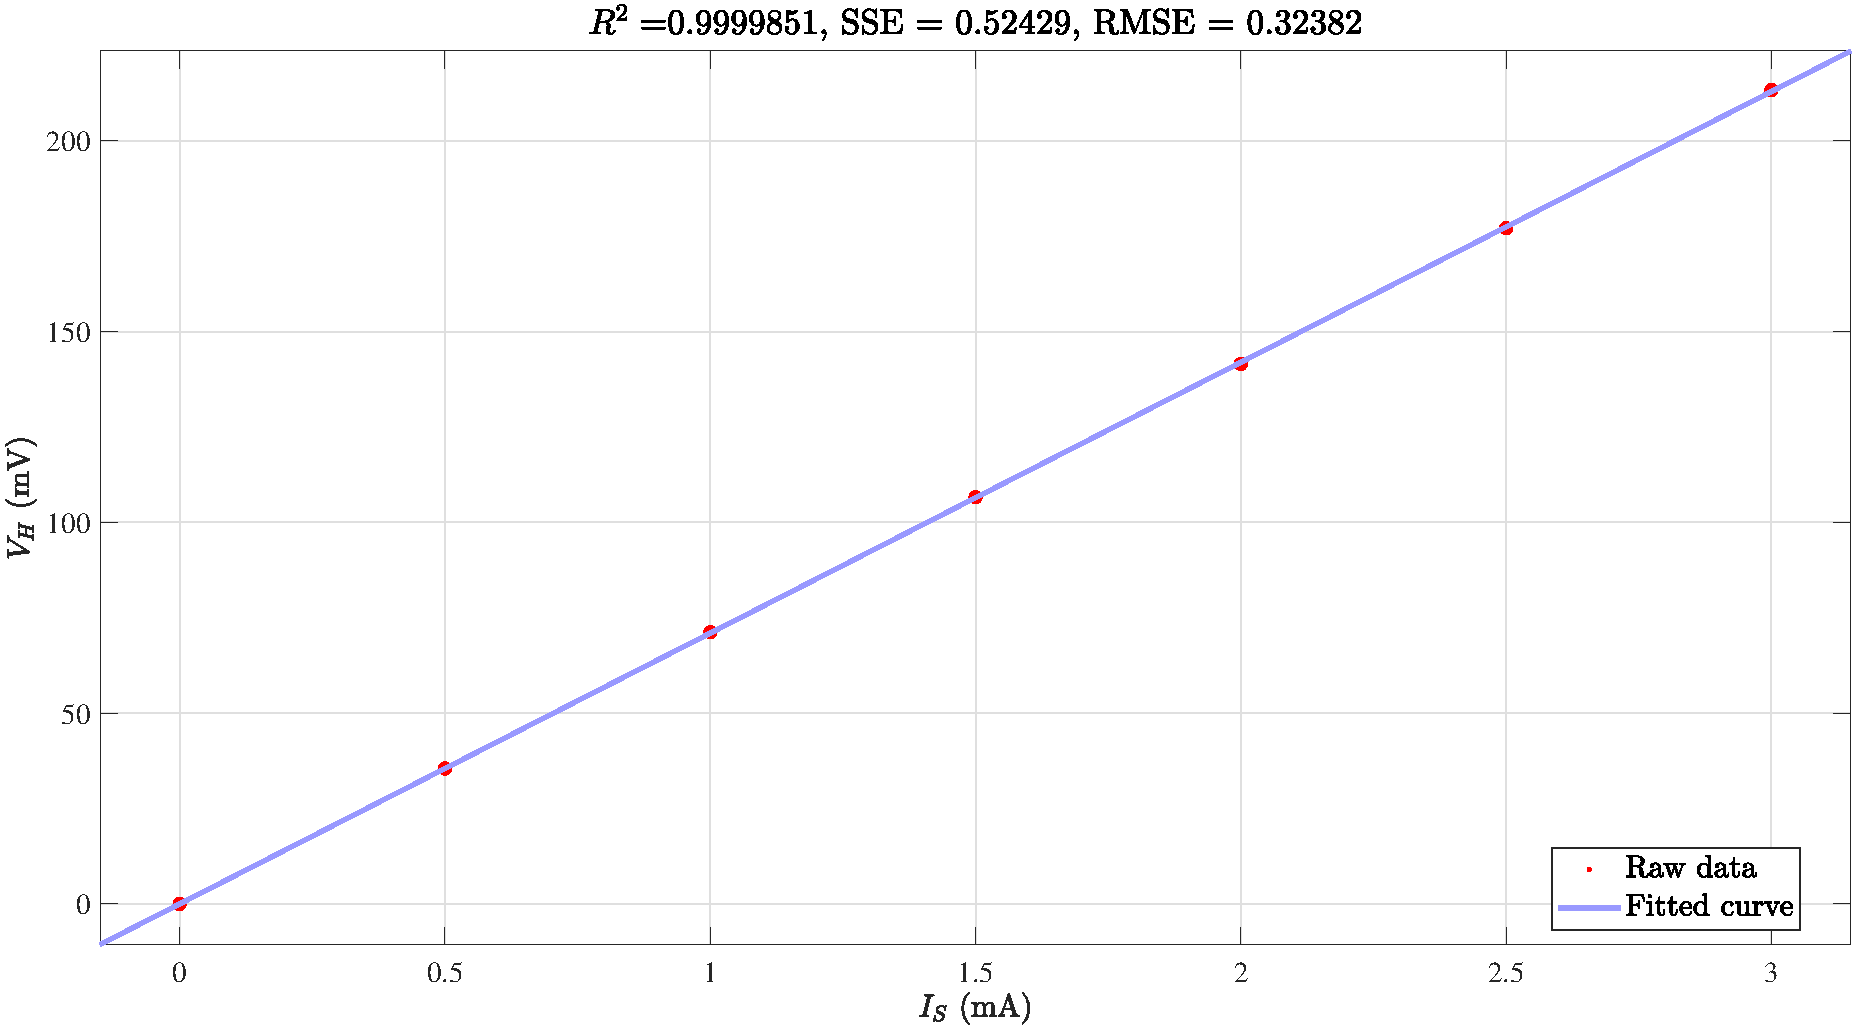
\includegraphics[width=8cm]{1.jpg}}\hspace{0.5cm}
    \subfigure[测量实验图像]{\includegraphics[width=8cm]{图片1.png}}
    \caption{ 铁氧体的饱和磁滞回线(竖直方向成对测量)}
\end{figure}

为了精准地从图像中得出所需$B_r$与$H_c$,将曲线单独描绘
并导入Get Data软件中读取坐标点(见图5):

\begin{figure}[htbp]
    \centering
    \includegraphics[width=12cm]{g1.png}
    \caption{铁氧体的饱和磁滞回线-数据获取}
\end{figure}
从右上角可以得到$B_r=0.074 $T(我将图中纵轴尺度放大了1000倍),$H_c=4.981 $(A/m)

\begin{center}
\large{5.2.1实验总结}
\end{center}

本实验相对比较简单,测量精确程度也比较高。
此外,拟合出的图像与理论预期符合地比较好,
成左右对称的形式(Get Data软件上的测量结果
显示$H_c=4.981,5.136$A/m,$B_r=0.074,0.076$T,可见相对误差还是比较小的)。


% % 左右两边的对称性并不足。
% % 在使用示波器时已经调制好了使其位于中间位置,
% % 但是还是不可避免地出现不对称的偏差,
% % 可能原因有:本身使用交流电来观察,就自然存在一定的不对称性,
% % 以及无法同时打开横纵坐标的原因。





\subsubsection{固定信号源幅度,观测并记录饱和磁滞回线随频率的变化规律}

保持$R_1,R_2,C$不变,测量并比较
$f=95\text{Hz}$和$f=150\text{Hz}$时的$B_r,H_c$.

由于诸参数并没有改变,
所以电压与所测物理量的换算关系仍然满足
\[
    H=\frac{N_1}{l R_1}u_{R_1}=\frac{150\times 10^{-3}}{0.130\times 2.0}u_{R_1}=\frac{15}{26}u_{R_1}\qquad
    B = \frac{R_2 C}{N_2 S}u_C=\frac{50\times 10.0\times 10^{-6}}{150\times 1.24\times 10^{-4}}=\frac {5}{186}u_c
\]
其中H的单位是A/m,$u_{R_1}$的单位是mV,B的单位是T,$u_C$的单位是mV.



测量数据见表2
(其中100Hz的数据为上一实验的结果,因为其余实验参量并没有改变,故可以使用):
\begin{table}[!ht]
    \centering
    \begin{tabular}{cccc}
        \toprule
        频率f & 95Hz&100Hz* & 150Hz \\ \midrule
        $U_{B_r}$/mV & 3.00 &-& 1.92 \\ 
        $U_{H_c}$/mV & 10.40&- & 4.80 \\ \midrule
        $B_r$/T & 0.081  &0.074& 0.052  \\ 
        $H_c$/(A/m) & 6.000 & 4.981& 2.769 \\ 
        \bottomrule
    \end{tabular}
    \caption{固定幅度下磁滞回线随频率的变化}
\end{table}

\begin{center}
    \large{5.2.2实验总结}
\end{center}

发现测量结果和预期符合地比较好。
但不足地是,我在测量过程中只采取了一侧,应该测量两侧数据并求均值,
不然可能会因为图像正负不够对称导致偏差。

*问题:用不同频率时,磁滞回线有何变化?为什么?

变化:频率增大,磁滞回线中$B_r,H_c$都不断减小,磁滞回线所围成的面积也随之减小,并且其光滑性增强,尖点减少。此外,反之,在频率减小到一定程度时,回线变得不清晰,波形不稳定。

原因:电路中存在电感$L$,增大频率,电感阻抗增大,因而分压增大,这就导致磁场测量部分的分压减小,因此各指标都呈减小趋势。






\subsubsection{在频率$f=50\text{Hz}$的情况下,比较不同积分常量取值对李萨如图形的影响}

固定励磁电流幅度$I_m=0.1\text{A},R_1=20\Omega$(方法是保持$u_1=I_m\times R_1=200$mV,这可以从示波器的网格中读出)
,改变积分常量$R_2C$。
调节分别为$0.01\text{s},0.05\text{s},0.5\text{s}$,
观察并记录下不同积分常量下李萨如图形的图。

我记录到的三个李萨如图形分别是(见图6-8):

\begin{figure}[H]
    \centering
    \includegraphics[width=11cm]{RC 0.5s.jpg}
    \caption{0.5s的情况}
\end{figure}

\begin{figure}[H]
    \centering
    \includegraphics[width=11cm]{RC 0.05s.jpg}
    \caption{0.05s的情况}
\end{figure}

\begin{figure}[H]
    \centering
    \includegraphics[width=11cm]{RC0.01S.jpg}
    \caption{0.01s的情况}
\end{figure}



\newpage
\begin{center}
    \large{5.2.3实验总结}
\end{center}

这个实验中$RC=0.5,0.05$s的两个图像记录得还比较准确,$RC=0.01$s的图像偏差得有些大(理论情况应该是原点处上下两侧接近于相切),
猜测出现失误的原因是频率波动(做实验的过程中我也发现,
有时调整实验电路的其他参量的时候,综合测量试验仪的输出频率会出现波动,我发现时都会手动调整回原来的频率,这里可能没有注意)。

但实际上,这三个李萨如图形对应着一个饱和磁滞回线,
但由于示波器的读取参量不同而图像有所不同,具体可见下面的问题与解答。

*问题:为什么积分常量会影响李萨如图形的形状?

原因:因为我们平常所说的(包括实验主要运用的),都是可以近似认为是积分常数远大于周期的情况。在积分常数为0.5s的时候是近似满足的,但是,当积分常数减小10倍甚至50倍之后,条件不再满足,故而李萨如图形的形状改变。

*问题:积分常量是否会影响真实的磁滞回线的形状?

答案:其实并不会。
因为积分常数只会影响比例,
进而影响其在示波器上的形状,
而示波器上其实并不会显示真实的磁滞回线的形状,
故而对真实磁滞回线形状并不影响。




\subsection{测量样品1(铁氧体)的动态磁滞回线}

在$f=100\text{Hz}$时,
取$R_1=2.0\Omega,R_2=50k\Omega,C=10.0\mu F$,测量20个顶点。

由于诸参数并没有改变,所以电压与所测物理量的换算关系仍然满足前面的换算式.

测得得的数据见表3:
\begin{table}[!ht]
    \centering
    \begin{tabular}{c|cc|ccc}
        \toprule
        数据点 & $U_x$/mV & $U_y$/mV & $H_m$/(A/m) & $B_m$/T & $\mu_m$ \\ \midrule
        1 & 1.84 & 0.40 & 1.062  & 0.011  & 8060.676  \\ 
        2 & 3.52 & 0.80 & 2.031  & 0.022  & 8427.070  \\ 
        3 & 6.96 & 1.60 & 4.015  & 0.043  & 8523.933  \\ 
        4 & 9.60 & 2.20 & 5.538  & 0.059  & 8497.296  \\ 
        5 & 13.4 & 3.40 & 7.731  & 0.091  & 9408.132  \\ 
        6 & 19.4 & 4.60 & 11.192  & 0.124  & 8791.954  \\ 
        7 & 22.8 & 5.80 & 13.154  & 0.156  & 9432.405  \\ 
        8 & 28.0  & 7.40 & 16.154  & 0.199  & 9799.479  \\ 
        9 & 32.8 & 8.20 & 18.923  & 0.220  & 9269.777  \\ 
        10 & 35.6 & 8.80 & 20.538  & 0.237  & 9165.622  \\ 
        11 & 40.8 & 10.0 & 23.538  & 0.269  & 9088.017  \\ 
        12 & 46.4 & 11.2 & 26.769  & 0.301  & 8950.130  \\ 
        13 & 52.0 & 12.2 & 30.000  & 0.328  & 8699.329  \\ 
        14 & 60.0 & 13.4 & 34.615  & 0.360  & 8281.001  \\ 
        15 & 72.0 & 14.8 & 41.538  & 0.398  & 7621.817  \\ 
        16 & 80.0 & 15.6 & 46.154  & 0.419  & 7230.426  \\ 
        17 & 94.4 & 16.6 & 54.462  & 0.446  & 6520.267  \\ 
        18 & 109 & 17.6 & 62.885  & 0.473  & 5987.085  \\ 
        19 & 124 & 18.4 & 71.538  & 0.495  & 5502.061  \\ 
        20 & 138 & 18.8 & 79.615  & 0.505  & 5051.357 \\ 
        \bottomrule
    \end{tabular}
    \caption{铁氧体的动态磁化曲线数据及处理}
\end{table}

由此绘制铁氧体的动态磁化曲线和$\mu_m -H_m$曲线如下(见图9与10):

\begin{figure}[H]
    \centering
    \includegraphics[width=14cm]{图片2.png}
    \caption{铁氧体的动态磁滞回线}
\end{figure}

\begin{figure}[H]
    \centering
    \includegraphics[width=14cm]{图片3.png}
    \caption{$\mu_m-H_m$磁化曲线}
\end{figure}

按照实验数据记录表上的建议,将二十个点的分配为前密后疏。还可以根据前期基础数据,
最后几个数据尽量调到最大的幅度(实验参量设置和第一个实验相同,
故可参考那里测得的$H=H_s$时的$U_x=122$mV与$U_y=18.4$mV)。

为了确定起始磁导率$$\displaystyle \mu_i=\lim_{H\to 0}\frac{B}{\mu_0 H}$$
 
我们关注H=0附近的曲线性态,于是选取前五个点,作拟合图如下:

\begin{figure}[H]
    \centering
    \includegraphics[width=12cm]{tie11.png}
    \caption{铁氧体的动态磁化曲线—H=0附近的性态图像}
\end{figure}

可以看到曲线拟合的相关系数$R^2=0.99415$,表明数据测量的合理性,进一步地
测得:
\begin{displaymath}\mu_i=\frac {11.87576\times 10^{-3}}{4\pi \times 10^{-7}}\approx 9.45 \times 10^3\end{displaymath}

\begin{center}
    \large{5.3实验总结}
\end{center}

可以发现,振幅磁导率$\mu_m=\frac{B_m}{\mu_0H_m}$随着电场强度的增加呈现降低的趋势,
这是因为样品越接近饱和磁化状态,增大磁场强度对磁感应强度的影响会变小。

再观察做得的两条曲线,
发现和理论上的预期结果相似,
说明找对了规律,
在误差范围内得到了相对比较正确的结论。

关于最后起始磁导率$\mu_i$的确定,如果取前四个数据点,会发现趋势线$y=10.80568x-0.56041$以相关系数$R^2=0.99993$的极高精度实现拟合。
可以算得$\mu_i\approx 8.59\times 10^{3}$,但四个数据点较少,故上述并没有选取这种方式并绘图。






\subsection{观察不同频率下样品2(硅钢)的动态磁滞回线}

参数调至$R_1=2.0\Omega,R_2=50k\Omega,C=10.0\mu F$,
在给定交变磁场幅度$H_m=400\text{A}/\text{m}$下,
测量三种频率的$B_m,B_r,H_c$.

尽管此时仪器参数没有改变,但样品2(硅钢)的参数发生了变化,需要取:
\[
    H=\frac{N_1}{l R_1}u_{R_1}=\frac{150\times 10^{-3}}{0.075\times 2.0}u_{R_1}=u_{R_1}\qquad
    B = \frac{R_2 C}{N_2 S}u_C=\frac{50\times 10.0\times 10^{-6}}{150\times 1.20\times 10^{-4}}=\frac{1}{36}u_c
\]
其中H的单位是A/m,$u_{R_1}$的单位是mV,B的单位是T,$u_C$的单位是mV.

根据实验的实际要求,先将$H_m$的值对应换算成所应观察的电压值,
换算得:$U=400\text{mA}$,
在示波器上调至格子为$200\text{mA}$的大小,
进行观察。
\newpage
做表如下,见表4:

\begin{table}[H]
    \centering
    \begin{tabular}{cccc}
        \toprule
        频率f & 20Hz & 40Hz & 60Hz \\ \midrule
        $U_{B_m}$/mV & 33.6 & 33.6 & 33.6 \\ 
        $U_{B_r}$/mV  & 19.2 & 21.6 & 22.4 \\ 
        $U_{H_c}$/mV  & 104 & 116 & 136 \\ \midrule
        $B_m$/T & 0.93  & 0.93  & 0.93  \\ 
        $B_r$/T& 0.53  & 0.60  & 0.62  \\ 
        $H_c$/(A/m) & 104.00  & 116.00  & 136.00 \\ 
        \bottomrule
    \end{tabular}
    \caption{不同频率下硅钢的动态磁滞回线参数}
\end{table}

\begin{center}
    \large{5.4实验总结}
\end{center}

可以看到,在不同频率的情况下,$B_m$基本不变化,而$B_r,H_c$逐渐变大。由此可以知道
硅钢的动态磁滞回线所围成的面积(也正相关于磁滞耗损)逐渐变大。
与之前的表2(固定幅度下铁氧体的磁滞回线随频率的变化数据表)做对比可以知道,二者的变化规律正好相反,
且硅钢的磁滞耗损更大——这些都和和理论的样品性质符合。

但是,
以统计规律来看的话,三组数据得到的结论还是比较粗糙,或许还需要更多的数据才可能下些断言。












\subsection{测量样品1(铁氧体)在不同直流偏置磁场下的可逆磁导率}

在$f=100\text{Hz}$时,
取$R_1=2.0\Omega,R_2=20k\Omega,C=2.0\mu F$,
直流偏置磁场从$0$到$H_s$单调递增,
测量10组回线小线段的斜率。

这一部分需要接入直流电源与电感,按照实验原理图(见图2),连接如下:
\begin{figure}[H]
    \centering
    \includegraphics[width=14cm]{直流偏置磁场.jpg}
    \caption{测量铁氧体在不同直流偏置磁场下的可逆磁导率:实验电路}
\end{figure}


这里参数$R_2$和$C$发生了变化,所以H和B的计算式要进行调整:
\begin{align*}
    &H=\frac{N_1}{l R_1}u_{R_1}=\frac{150\times 10^{-3}}{0.130\times 2.0}u_{R_1}=\frac{15}{26}u_{R_1}\\
    &B = \frac{R_2 C}{N_2 S}u_C=\frac{20\times 2.0\times 10^{-6}}{150\times 1.24\times 10^{-4}}=\frac{1}{465}u_c\\
    &H_{out}=\frac{N_3}{l}i=\frac{15000}{13}i
\end{align*}
其中H的单位是A/m,$u_{R_1}$的单位是mV,B的单位是T,$u_C$的单位是mV,i的单位是A

为了更加精确地得到可逆磁导率,我测量了第一象限和第三象限地端点坐标$(H_1,B_1)$,
计算可得表5:
\begin{table}[H]
    \centering
\begin{tabular}{c|ccccc|cccc}
    \toprule
    数据点 & 电流I/A & $U_{x_1}$/mV & $U_{y_1}$/mV & $U_{x_3}$/mV & $U_{y_3}$/mV & $H_1$/(A/m) & $B_1$/mT & $H_3$/(A/m) & $B_3$/mT \\ \midrule
    1 & 0.01 & 7.60 & 13.2 & -7.20 & -12.4 & 4.385  & 28.387  & -4.154  & -26.667  \\ 
        2 & 0.02 & 15.2 & 19.2 & -12.8 & -18.4 & 8.769  & 41.290  & -7.385  & -39.570  \\ 
        3 & 0.03 & 14.0 & 13.6 & -12.4 & -12.0 & 8.077  & 29.247  & -7.154  & -25.806  \\ 
        4 & 0.04 & 22.4 & 16.0 & -18.4 & -14.4 & 12.923  & 34.409  & -10.615  & -30.968  \\ 
        5 & 0.05 & 26.4 & 13.6 & -22.4 & -12.4 & 15.231  & 29.247  & -12.923  & -26.667  \\ 
        6 & 0.06 & 36.8 & 12.8 & -28.0 & -12.0 & 21.231  & 27.527  & -16.154  & -25.806  \\ 
        7 & 0.08 & 48.8 & 10.4 & -37.6 & -9.60 & 28.154  & 22.366  & -21.692  & -20.645  \\ 
        8 & 0.10 & 52.0 & 6.40 & -38.0 & -5.60 & 30.000  & 13.763  & -21.923  & -12.043  \\ 
        9 & 0.12 & 46.4 & 3.60 & -42.4 & -3.20 & 26.769  & 7.742  & -24.462  & -6.882  \\ 
        10 & 0.14 & 45.6 & 2.80 & -43.2 & -42.4 & 26.308  & 6.022  & -24.923  & -91.183  \\ 
        11 & 0.16 & 43.2 & 2.00 & -42.4 & -1.20 & 24.923  & 4.301  & -24.462  & -2.581  \\ 
        12 & 0.18 & 42.4 & 1.60 & -41.6 & -0.80 & 24.462  & 3.441  & -24.000  & -1.720  \\ 
        13 & 0.20 & 41.6 & 1.20 & -40.8 & -0.40 & 24.000  & 2.581  & -23.538  & -0.860 \\ 
    \bottomrule
\end{tabular}
\caption{铁氧体在不同直流偏置磁场下的可逆磁导率数据及处理}
\end{table}

并取前八组数据的一三象限数据分别处理,同一参量下获得的可逆磁导率$\mu_R$加以平均,得到$\overline \mu_R$:
\begin{table}[H]
    \centering
    \begin{tabular}{ccccc}
        \toprule
        数据点&$H_{out}$/(A/m) & $\mu^1_{R}$ & $\mu_{R}^3$ & $\overline \mu_R$ \\ \midrule
        1&11.538  & 5152.045  & 5108.677  & 5130.361  \\ 
        2&23.077  & 3746.942  & 4264.097  & 4005.520  \\ 
        3&34.615  & 2881.576  & 2870.641  & 2876.109  \\ 
        4&46.154  & 2118.806  & 2321.475  & 2220.140  \\ 
        5&57.692  & 1528.109  & 1642.075  & 1585.092  \\ 
        6&69.231  & 1031.767  & 1271.284  & 1151.525  \\ 
        7&92.308  & 632.168  & 757.361  & 694.764  \\ 
        8&115.385  & 365.087  & 437.143  & 401.115 \\ 
        \bottomrule
    \end{tabular}
    \caption{数据处理:可逆磁导率与直流偏置磁场强度}
\end{table}

此时就可以作出外场与可逆磁导率的关系图(如图13)。
利用曲线拟合,
发现在可逆磁导率$\mu_R$的数值随直流偏置磁场强度的增加而单调减少,
并且我们注意到,趋势线\[
    \mu_R=6844.2260536\mathrm e^{0.0248585}H
\]
以$R^2=0.9985856$的高精度拟合测量曲线,从$H=10\backsim 120$A/m区间的拟合效果
都很好,从而可以得到可逆磁导率:$$\mu_R\approx 6844.23$$

\begin{figure}[H]
    \centering
    \includegraphics[width=14cm]{图片4.png}
    \caption{可逆磁导率与直流偏置磁场的关系图}
\end{figure}

\begin{center}
    \large{5.5实验总结}
\end{center}

本次实验有个小失误:因为实验数据记录表上要求"直流偏置磁场从0到$H_s$单调增加",即要控制
直流电源的输出电流i均匀单调增加。我最开始采取0.02mA作为电流增长幅度,但实验数据(见表5)表明在i=0.12mA及以后的状态下
$U_x,U_y$变化幅度很小,若采取这段数据处理,会导致实验误差较大。故我又补测了i=0.01、0.03、0.05mA下的实验数据,也算把这一失误弥补了。
这也是上述作表6时只采取了前8个数据点的原因。


可以看到,随着外加磁场强度的增强,
其磁导率呈单调递减之势,符合实验预期。
且在最后时,其减少趋势减缓(即其导数的绝对值减小,逐渐趋于0),
最后预测将会趋于稳定状态,符合理论结果。

不过,事实上,虽然数据已经比较相近,
但仍有不小的误差。
其原因可能主要是由于在实际实验过程中无论如何也做不到在趋
近于零的范围内进行测量,只能通过拟合的方式去估计值,
导致不够“微分”,变化不够微小,
因而误差较大;此外,
实验仪器本身的误差也导致无法测准。








\subsection{测量模具钢样品的起始磁化曲线}

将霍尔传感器位于磁场均匀区(这需要事先探测均匀的范围,我测到的为0.0-0.4mm区域)
中央,取20个采样点,测量样品的起始磁化曲线。

成功进行退磁处理(方法是利用双刀开关使磁化电流不断反向,并逐次减小幅值大小)
后,进行正式实验。

\begin{figure}[H]
    \centering
    \includegraphics[width=11cm]{huoer.jpg}
    \caption{即将完成退磁过程时的实验电路}
\end{figure}



原始的$I,B$均可以在实验室测得,
而$H$则依靠公式:\begin{displaymath}H=\frac{N}{\bar{l}}I\end{displaymath}
以及:\begin{displaymath}\text{ 修正 } H=\frac{NI}{\bar{l}}-\frac{Bl_g}{\mu_0{\overline l}}\end{displaymath}进行计算。
其中$N=2000$为总匝数,
$\bar{l}=0.240\text{m}$为平均磁路长,
$l_g=2\times 10^{-3}\text{m}$为缝隙宽度,

列表见表7:
\begin{table}[H]
    \centering
    \begin{tabular}{ccccc}
        \toprule
        数据点 & 电流I(mA) & B(mT) & H(A/m) & $H_{cor}$ (A/m)\\ \midrule
        1 & 0.0 & -0.5 & 0.00  & 0.80  \\ 
        2 & 30.1 & 9.2 & 250.83  & 236.19  \\ 
        3 & 60.4 & 20.7 & 503.33  & 470.39  \\ 
        4 & 90.5 & 33.8 & 754.17  & 700.37  \\ 
        5 & 119.7 & 47.6 & 997.50  & 921.74  \\ 
        6 & 148.6 & 63.8 & 1238.33  & 1136.79  \\ 
        7 & 179.3 & 79.9 & 1494.17  & 1367.00  \\ 
        8 & 209.8 & 99.3 & 1748.33  & 1590.29  \\ 
        9 & 238.4 & 119.6 & 1986.67  & 1796.32  \\ 
        10 & 271.9 & 145.1 & 2265.83  & 2034.90  \\ 
        11 & 298.7 & 165.4 & 2489.17  & 2225.92  \\ 
        12 & 328.9 & 187.4 & 2740.83  & 2442.58  \\ 
        13 & 359.0  & 208.9 & 2991.67  & 2659.19  \\ 
        14 & 388.6 & 229.6 & 3238.33  & 2872.91  \\ 
        15 & 420.8 & 251.9 & 3506.67  & 3105.76  \\ 
        16 & 451.6 & 272.7 & 3763.33  & 3329.32  \\ 
        17 & 480.6 & 291.4 & 4005.00  & 3541.22  \\ 
        18 & 511.8 & 310.3 & 4265.00  & 3771.14  \\ 
        19 & 538.6 & 325.6 & 4488.33  & 3970.12  \\ 
        20 & 571.4 & 342.8 & 4761.67  & 4216.08 \\ 
        \bottomrule
    \end{tabular}
    \caption{霍尔传感器测量样品的起始磁化曲线}
\end{table}

其磁化曲线见图15:

\begin{figure}[H]
    \centering
    \includegraphics[width=12cm]{图片5.png}
    \caption{模具钢的起始磁化曲线}
\end{figure}

\begin{center}
    \large{5.6实验总结}
\end{center}



该部分实验较为成功,成功拟合出了大致的磁化曲线,且在调节电路时距离60的整数倍较小,误差较小。比较符合真实情况。

但是,需要关注的是,受设备限制,即便采样到电流峰值633.3mA,
磁化强度也仅略显平稳,每增加10mA电流,仍然显示出几mT的增加。
故实际操作中不能达到饱和磁化状态。





\subsection{测量模具钢的磁滞回线}

电流$I_m$减少到0,再反向增大到$-I_m$再减回0,再反向增大到$I_m$即可。

计算和修正H的办法同5.6小节。

原始数据及处理数据见表8。

\begin{table}[!ht]
    \centering
    \begin{tabular}{ccccc|ccccc}
        \toprule
        数据点 & 电流I(mA) & B(mT) & H(A/m) & $H_{cor}$(A/m) & 数据点 & 电流I(mA) & B(mT) & H(A/m) & $H_{cor}$(A/m)\\ \midrule
        1 & 571.4 & 354.0 & 4761.67  & 2414.13  & 26 & -545.3 & -332.4 & -4544.17  & -2339.87  \\ 
        2 & 520.2 & 346.6 & 4335.00  & 2036.54  & 27 & -497.1 & -325.0  & -4142.50  & -1987.28  \\ 
        3 & 470.9 & 338.5 & 3924.17  & 1679.42  & 28 & -449.7 & -316.5 & -3747.50  & -1648.64  \\ 
        4 & 417.4 & 327.9 & 3478.33  & 1303.88  & 29 & -398.4 & -305.4 & -3320.00  & -1294.75  \\ 
        5 & 381.6 & 319.4 & 3180.00  & 1061.91  & 30 & -356.9 & -294.4 & -2974.17  & -1021.87  \\ 
        6 & 335.4 & 306.1 & 2795.00  & 765.11  & 31 & -295.1 & -273.5 & -2459.17  & -645.46  \\ 
        7 & 281 & 286.1 & 2341.67  & 444.41  & 32 & -245.2 & -251.2 & -2043.33  & -377.51  \\ 
        8 & 231.6 & 262.8 & 1930.00  & 187.25  & 33 & -198.4 & -225.6 & -1653.33  & -157.28  \\ 
        9 & 183 & 235.0  & 1525.00  & -33.39  & 34 & -155.5 & -198.4 & -1295.83  & 19.85  \\ 
        10 & 130.7 & 200.4 & 1089.17  & -239.78  & 35 & -105.4 & -163.4 & -878.33  & 205.25  \\ 
        11 & 76.6 & 161.3 & 638.33  & -431.32  & 36 & -63.4 & -132.4 & -528.33  & 349.67  \\ 
        12 & 29.1 & 125.1 & 242.50  & -587.10  & 37 & 0.0 & -83.2 & 0.00  & 551.74  \\ 
        13 & 0.0 & 102.2 & 0.00  & -677.73  & 38 & 44.0 & -47.8 & 366.67  & 683.65  \\ 
        14 & -50.4 & 61.5 & -420.00  & -827.83  & 39 & 98.6 & -2.9 & 821.67  & 840.90  \\ 
        15 & -103.1 & 18.0 & -859.17  & -978.53  & 40 & 151.0 & 40.7 & 1258.33  & 988.43  \\ 
        16 & -149.2 & -20.4 & -1243.33  & -1108.05  & 41 & 196.6 & 78.7 & 1638.33  & 1116.44  \\ 
        17 & -204.7 & -66.5 & -1705.83  & -1264.84  & 42 & 246.9 & 119.3 & 2057.50  & 1266.37  \\ 
        18 & -255.0  & -106.8 & -2125.00  & -1416.76  & 43 & 301.0 & 161.9 & 2508.33  & 1434.70  \\ 
        19 & -298.2 & -140.6 & -2485.00  & -1552.62  & 44 & 358.4 & 205.6 & 2986.67  & 1623.24  \\ 
        20 & -347.2 & -178.2 & -2893.33  & -1711.61  & 45 & 398.6 & 235.1 & 3321.67  & 1762.61  \\ 
        21 & -407.0  & -221.8 & -3391.67  & -1920.81  & 46 & 447.9 & 269.3 & 3732.50  & 1946.65  \\ 
        22 & -462.6 & -259.7 & -3855.00  & -2132.81  & 47 & 501.8 & 303.7 & 4181.67  & 2167.69  \\ 
        23 & -500.6 & -283.8 & -4171.67  & -2289.66  & 48 & 552.1 & 332.3 & 4600.83  & 2397.20  \\ 
        24 & -545.8 & -310.3 & -4548.33  & -2490.59  & 49 & 596.3 & 354.5 & 4969.17  & 2618.32  \\ 
        25 & -603.1 & -340.2 & -5025.83  & -2769.81  & 50 & 631.9 & 370.5 & 5265.83  & 2808.88 \\ 
        \bottomrule
    \end{tabular}
    \caption{霍尔传感器测量:样品模具钢的饱和磁滞回线数据}
\end{table}

由此,作图绘出的磁滞回线为图16。

\begin{figure}[H]
    \centering
    \includegraphics[width=12cm]{图片6.png}
    \caption{模具钢的饱和磁滞回线}
\end{figure}

\begin{center}
    \large{5.7实验总结}
\end{center}

该实验也比较成功,得到的曲线形状准确,且对于中心的偏离较小。
由于电流i、$B$的测量准确度较高,因而$H$修正值的准确程度也不低,
加上做实验之前我对样品的磁锻炼比较充分(细节:拉动
开关后,应使触点从接触到断开的时间长一些,保证材料在当前磁场中稳定磁化),而且数据比较精确,整体实验较为成功。

另外,在做实验之前,我预习实验讲义的过程中,很好奇$H$的修正对最终磁滞回线的形状的影响。
原本以为修正与否只会造成比较微小的差别,但实际上,$H_{cor}$相对于$H$完全不同!这可从上面的表8或者
下面展示的两个实验修正前后图像对比图可知:


\begin{figure}[H]
    \centering
    \subfigure[起始磁化曲线]{\includegraphics[width=12cm]{图片8.png}}
    \subfigure[(准)静态磁滞回线]{\includegraphics[width=12cm]{图片9.png}}
    \caption{霍尔传感器测量下模具钢样品的实验图像—H修正前后对比}
\end{figure}

这也告诉我们,在做实验或者实验后处理数据的过程中,不能想当然地忽略一些因素,
应该就实验具体形式和数据来源等予以全面地考虑。

\newpage
\section{思考题}
*实验数据记录表和实验讲义上的一些问题,已经在每小节的{\bf 实验总结}中解答,不再重复。

\begin{enumerate}

    \item 思考题1:  \textbf{铁磁材料的动态磁滞回线与(准)静态磁滞回线在概念上有什么区别?铁磁材料动态磁滞回线的形状和面积受那些因素影响?}

区别:铁磁材料的动态磁滞回线是在交变电场的作用下,
得到的$B-H$关系曲线,而静态磁滞回线仅记录了磁化完全后的$B-H$关系曲线。

影响因素:(1)动态磁滞回线受到铁磁材料种类、
大小、交流电频率和振幅等多种因素的影响,
其围成的面积等于一个周期的能量损耗,
其除了磁滞损耗外,还包括涡流损耗、剩余损耗,
它们也受多种因素影响。(2)静态磁滞回线因为没有磁场大小随时间的变化,
因此几乎没有涡流损耗和剩余损耗,基本上就是磁滞损耗。

    \item 思考题2:  \textbf{什么叫做基本磁化曲线?它和起始磁化曲线间有何区别?}

    对于一个处于磁中性状态(H=0 ,且B=0)的铁磁材料加上由小变大的磁场
     H 进行磁化时,磁感应强度 B 随 H 的变化曲线称为起始磁化曲线。
     
     如果对绕上磁化线圈的铁磁材料样品施加直流激励,
     便会在样品中产生稳定的磁场。
     当直流激励的大小发生变化,H 与 B 也随之改变,
     形成磁化曲线和磁滞回线。
     
     如果在样品的磁路中开一极窄均匀气隙,
     在对磁化线圈中的磁化电流最大值Im磁锻炼的基础上,
     对应每个磁化电流 Ik值,用数字式特斯拉计,
     测量气隙均匀磁场区中间部位的磁感应强度B,
     便能得到该磁性材料的磁滞回线。对于一定大小的回线,
     磁化电流最大值设为Im,对于每个不同的Ik值,使样品反复磁化,
     可以得到一簇磁滞回线。
     把每个磁滞回线的顶点以及坐标原点 O 连接起来,
     得到的曲线称基本磁化曲线。这两者有明显的区别。

    或者简单来说,基本磁化曲线是不同的静态磁滞回线的顶点、
坐标原点相连形成的曲线。
后者是一族(多条)动态磁滞回线的顶点、与
坐标原点相连形成的新曲线。

    \item 思考题3:  \textbf{铁氧体和硅钢材料的动态磁化特性各有什么特点?}

铁氧体材料比硅钢材料更容易磁化且其磁导率更高,矫顽力更小,
因此磁滞损耗也更小。
同时,铁氧体单位体积中存储的磁能更低,饱和磁化强度也更低。
相反,硅钢材料磁导率低,磁化难,矫顽力大,需要更大的磁场才能让材料的磁性逆转。

且随频率的增大,二者表现出的特性也不同——铁氧体磁滞耗损变小而硅钢的增大。
也因此,硅钢片通常用于低频变压
器而铁氧体通常用于高频变压器。
这些可以从实验5.2.1、5.2.2、5.4中观察到。

    \item 思考题4:  \textbf{动态磁滞回线测量实验中,电路参量应怎样设置才能保证$u_{R_1}-u_C$所形成的李萨如图形正确反映材料动态磁滞回线的形状?}

一方面,应该满足积分常数$R_2C>>T$(其中$T$是输入信号的周期尺度),
这是推导公式(推导公式$B=\frac{R_2 C}{N_2 S}u_c$时,需要用到积分近似$u_c=\frac{1}{R_2 C}\int u_2\mathrm d t$,这里就要要求$R_2C>>T$)
是所满足近似关系的必要条件;
此外,从另一方面来说,交流电幅度应当充分大,
以便于铁磁体饱和磁化。

主要就是受到这两个实验参量的影响。如果达不到上面的要求,
所观察到的磁滞回线可能变形,
与真实的动态磁滞回线有较大差别,从实验5.2.3中也可以看到这一点。


    \item 思考题5:  \textbf{准静态磁滞回线测量实验中,为什么要对样品进行磁锻炼才能获得稳定的饱和磁滞回线?}
    
    磁锻炼,即反复进行正反向饱和磁化,
    可以消除磁介质中剩有的磁阻力,使得磁介质接近饱和,得到一
个中心对称的饱和磁滞回线。
    
    对同一外磁场$H_m$,由于磁化历史会导致在磁化与退磁过程中产生不同的剩磁,
    其所对应的$B_m$值也不同,
    因此需要多次循环磁化直到$B_m$稳定,此时才能出现闭合、稳定的磁滞回线。

    
\end{enumerate}



\newpage
\section{实验感想总结}

本次实验分为两个部分——首先是利用磁特性综合测量实验仪的电路设计将磁感应强度、
磁场强度等磁学量转化为电信号,并用示波器使之可视化,并进一步进行一系列地观测;
其次是利用霍尔传感器测量并绘制铁磁材料的静态磁滞回线。本次实验还针对两种风格特异的实验仪器,
安排了退磁技术和“磁锻炼”部分,作为一个重要的部分嵌入其中,
丰富了实验的内容,增加了趣味性。

本次实验总体上是成功的——我成功测得了铁氧体和硅钢样品$B_r,H_c$等磁滞回线的重要特征量随频率f的变化趋势,
测得了铁氧体的饱和磁滞回线、动态磁化曲线,观察了不同积分常量$R_2 C$对李萨如图形的影响(尽管$R=0.01$s的李萨如图形记录得有些偏差),
测量了不同种类的磁导率,测量并描绘了模具钢的起始磁化曲线和动态磁滞回线……实验内容丰富,实验数据精度较高,实验图像与理论总体符合较好。

数据测量结束并不意味着实验的结束——如何进行数据的处理、图像的绘制和拟合、实验现象的分析解释、实验误差的来源阐释、实验报告的规范撰写等等都是
"物理实验"的重要组成部分。本次实验中我用Excel作数据的处理计算,对基本操作的熟悉外还新学习了如何绘制多横轴图像以及一些快捷函数的调用;用新配置的\LaTeX 撰写实验报告,
内容、公式等的呈现更为规范;利用Get Data软件读取图像数据点,最大限度降低二次误差的产生;结合实验讲义以及我的知识贮备、实验过程中的观察等多方面的信息进行实验结果的分析展示(见每一小节的实验总结);
以及按照李老师和物理实验总的要求认真撰写实验报告。

本次实验我还收获到了:

其一,还是预习的重要性。本次实验的高效完成离不开前期对实验讲义的琢磨与解读。

其二,体会到数据处理的重要性。这个实验很多数据是原始的,不能只能拿来绘图等进行直接采用的,而且数据的修正对结果的影响超出了我的预期。
因而掌握对原始数据的正确处理,也是我们学习的必修课。

其三,体会到物理“理论同实验结合”的学科魅力与特色。归根结底,物理是一门实验学科,对它的学习如果只是
从书本上看,从课堂上听,而没有动手亲自“学”的话,终究对其的理解和把握是有限的。磁滞回线的相关概念已经比较熟悉,
但真正像这样动手测量一遍并绘制相关图像的过程中,对它们的认识又加深了一层。
当漂亮对称的饱和磁滞回线展示在面前时,心中难免充满喜悦和感慨。

——————————

附:

1、预习实验报告(手写pdf版导入)

2、原始实验数据记录表(包含老师签名)(扫描为pdf版导入)

\newpage

\includepdf[pages={1-2}]{CZ预习实验报告.pdf}
\includepdf[pages={1-4}]{czhysj.pdf}


\end{document}